\chapter{Algorithmen und Implementierung}
\label{cha:Algorithmen und Implementierung}

Wir werden in diesem Kapitel den Algorithmus des Heuristik Agenten und des TD-Q-Agenten betrachten. Nachfolgend haben wir die wichtigsten Algorithmen für die Implementierung der Agenten dargestellt und erläutert. Die Gesamtheit aller für die Implementierung nötigen Algorithmen und der Tests findet man auf der beiliegenden Software-CD. \\

Für die Konvergenz des TD-Q-Lernens ist die Theorie des Erkundens und Verwertens (eng. exploration and exploitation) elementar wichtig. Am Ende des Kapitels werden wird dazu näheres erklären. \\

Weiterhin beschreiben wir am Ende des Kapitels, wie wir einen Spielzustand in einen einzigartigen Zahlenwert (Hash-Wert) umwandeln können, d.h. jede unterschiedliche Spielsituation wird durch einen anderen Zahlenwert referenziert. Wir benötigen diese einzigartige Referenzierung für das speichern und aktualisieren der Q-Werte in einer Datenbank. \\

Die von mir implementierten Algorithmen sind in der Programmiersprache Python realisiert. Python ist eine Hochsprache, die sehr leicht erlernbar ist und leicht von Menschen gelesen werden kann. Sie ähnelt einer Darstellung in Pseudocode. Python wird außerdem sehr gerne im Bereich des maschinellen Lernens eingesetzt. Wir verwenden in dieser Arbeit die Python Version 2.7.13. \\
\newpage

\section{Iterative-Alpha-Beta-Suche}
Die Alpha-Beta-Suche und die iterativ vertiefende Tiefensuche des Abschnitts waren bereits Thema im Abschnitt \ref{cha:Realisierung des Heuristik Agenten}. Es folgt eine Beschreibung der Implementierung dieser beiden Algorithmen.\\

Sehen wir uns das Codebeispiel aus Abbildung \ref{fig:Alpha-Beta iterativ vertiefende Suche} genauer an. Der Eingabeparameter der Funktion ist ein Zustand (eine Spielsituation) der Spielumgebung. Basierend auf diesem Zustand expandiert die Funktion einen Suchbaum mit der maximalen Tiefe 2. Ziel der Funktion ist es, ein minimales oder ein maximales Ergebnis innerhalb der Suchtiefe 2 zu finden. Muss der Kreuzspieler seinen Spielzug ausführen, dann wird ein maximales Ergebnis gesucht und muss der Kreisspieler seinen Spielzug ausführen, wird ein minimales Ergebnis gesucht. Zurückgegeben wird ein entsprechendes Aktionstupel der Form (x,y) oder der Form (Koordinate 1, Koordinate 2). \\

Das Codebeispiel bezieht sich auf die Tic Tac Toe Implementierung der iterative vertiefenden Alpha-Beta-Suche. Die Reversi Implementierung ist fast identisch. Einzig der Vergleich in Zeile 8 ist unterschiedlich. Würde dieser Vergleich ausgelagert werden, wären die Algorithmen identisch, denn die Funktionalitäten der Strategiespielumgebungen sind sehr ähnlich definiert. \\

\begin{figure}[!htbp]
\centering
\begin{lstlisting}[frame=single, mathescape=true]
1  def alphaBetaIterativeDeepeningSearch(state):
2    listOfActionUtilities = []
3    actionList = actions(state)
4    for action in actionList:
5      state.makeMove(action)
6      listOfActionUtilities.append(maxValue(
         state, -sys.maxint, sys.maxint, 0, 2))
7      state.undoMove()
8    if state.getPlayerToMove() == 'X':
9      bestActionIndex = argmax(listOfActionUtilities)
10   else:
11     bestActionIndex = argmin(listOfActionUtilities)
12   return actionList[bestActionIndex]
\end{lstlisting}
\caption{Codeauszug der Iterativen-Alpha-Beta-Suche.}
\label{fig:Alpha-Beta iterativ vertiefende Suche}
\end{figure} 
\newpage

Die in der Funktion alphaBetaIterativeDeepeningSearch(state) verwendete Funktion maxValue(state, alpha, beta, depth, depthBound), realisiert die rekursive Exploration des Suchbaums (siehe Abbildung \ref{fig:Iteratives Suchen des maximalen Ergebnisses}). Die Funktion liefert den Ergebniswert eines Spielzustands, dieser wird durch die Bewertungsfunktion evaluate(state) bestimmt. Die Rekursion entsteht durch den Aufruf der Funktion minValue(state, alpha, beta, depth +1, depthBound). Der Eingabeparameter ''depth + 1'' bedeutet eine Erhöhung der aktuellen Tiefe. Der Eingabeparameter ''depthBound'' speichert die maximale Tiefe, die von der aktuellen Tiefe nicht überschritten werden darf. Die beiden Funktionen minValue(...) und maxValue(...) unterscheiden sich nur in ihren letzten drei Codezeilen und in dem gegenseitigen Aufrufen der jeweils anderen Funktion. Die letzten drei Codezeilen von minValue(...) bewirken: Liefere Alpha zurück, wenn $Beta <= Alpha$ ist, andernfalls gib Beta zurück. \\

Die beiden Codebeispiele (Abbildung \ref{fig:Alpha-Beta iterativ vertiefende Suche} und Abbildung \ref{fig:Iteratives Suchen des maximalen Ergebnisses}) sind abgeleitet vom Alpha-Beta Algorithmus \cite[214 \psq]{Russell} und dem Algorithmus der iterativ vertiefenden Tiefensuche \cite[124]{Russell}.\\

\begin{figure}[!htbp]
\centering
\begin{lstlisting}[frame=single, mathescape=true]
1  def maxValue(state, alpha, beta, depth, depthBound):
2    if cutoffTest(state, depth, depthBound):
3      return evaluate(state)
4    for a in actions(state):
5      state.makeMove(a)
6      alpha = max(alpha, minValue(
         state, alpha, beta, depth + 1, depthBound))
7      state.undoMove()
8      if alpha >= beta:
9        return beta
10   return alpha
\end{lstlisting}
\caption{Iteratives Suchen des maximalen Ergebnisses.}
\label{fig:Iteratives Suchen des maximalen Ergebnisses}
\end{figure} 

\newpage

\section{TD-Q-Lernen}
Das Thema in diesem Kapitel ist die Implementierung des TD-Q-Lernens und die Erläuterung des dafür benötigten Algorithmus. \\

\begin{figure}[!htbp]
\centering
\begin{lstlisting}[frame=single, mathescape=true]
1  def Q-Lernen(s', r', $\alpha$, $\gamma$):
2    if istTerminalzustand(s):
3      Q[s, None] $\leftarrow$ r'
4    if s ist nicht None:
5      inkrementiere $N_{sa}$[s, a]
6      Q[s, a] $\leftarrow$ Q[s, a] + $\alpha$(N$_{sa}${s, a])
  		* (r + $\gamma max_{a'}$ Q[s', a'] - Q[s, a])
7    s, a, r $\leftarrow$ s', argmax$_{a'}$, f(Q[s', a'], N$_{sa}$), r'
8    return a
\end{lstlisting}
\caption{Algorithmus des TD-Q-Lernens vgl. \cite[974]{Russell}}
\label{fig:TD-Q-Lernen Algorithmus}
\end{figure} 

Der Q-Lernen Algorithmus (Abbildung \ref{fig:TD-Q-Lernen Algorithmus}) verwendet einige persistente (d.h. beständige oder dauerhafte) Variablen. Persistent deshalb, weil sie die einzelnen Funktionsaufrufe bzw. Iterationen des Algorithmus überdauern:
 
\begin{itemize}
\item \textbf{Q} ist eine Tabelle mit Aktionswerten, indiziert nach Zustand und Aktion. Der Aufruf Q[s, a] liefert z.B. einen Aktionswert (Q-Wert) für eine Aktion a in einem Zustand s. Zu Beginn des Lernprozesses sind alle Werte dieser Tabelle leer. Die Abbildung von Zustand/Aktionspaaren auf Nutzenwerte wird als Q-Funktion bezeichnet. Für die Realisierung einer solchen Q-Tabelle bzw. Q-Funktion implementieren wir diverse SQLite Datenbank Funktionen, um diese Datenbankfunktionen zu verwirklichen benutzen wir benutzen wir das Python Paket ''sqlite3''. Die Datenbank Funktionen erstellen und aktualisieren Q-Werte, der Zugriff auf diese Q-Werte erfolgt wie bereits beschrieben durch Zustand/Aktionspaare.

\item \textbf{N$_{sa}$} ist eine Tabelle mit Häufigkeiten für Zustand/Aktions-Paare.  Diese ist wie Q anfangs leer. Jedes mal wenn ein Zustand/Aktions-Paar durchlaufen wird, welches bereits durchlaufen wurde, dann wird der Tabelleneintrag N$_{sa}$[s, a] inkrementiert d.h. um den Wert 1 erhöht. Anstatt diese Statistik über bereits besuchte Zustand/Aktionspaare zu führen, verwenden wir eine geeignete Explorationsfunktion f (später im aktuellen Abschnitt erklärt).
\newpage

\item \textbf{s} ist der vorhergehende Spielzustand (eine Instanz der Strategiespielumgebungen), anfangs leer. Berücksichtigen wir den zeitlichen Aspekt, dann wäre s zu einem Zeitpunkt t geschrieben s${_t}$ und ein darauffolgender Spielzustand wäre s${_t+1}$. Der direkt auf s folgende Spielzustand wird auch als s' (s Prime) bezeichnet.

\item \textbf{a} ist die vorhergehende Aktion (ein Positionstupel der Spielmatrix), anfangs leer. Wird die Aktion a im Zustand s ausgeführt, dann wird der Zustand s' bzw. s$_{t+1}$ erreicht. Eine Aktion die in s' ausgeführt werden kann, bezeichnen wir als a' oder a$_{t+1}$.

\item \textbf{r} ist die Belohnung, die dem Agenten von der Umgebung zugeteilt wird, anfangs leer, wenn der Agent eine Aktion a in einem Zustand s ausführt (die Funktion der Strategiespielumgebung getReward() liefert diesen Wert). Wir können eine Funktion r(s, a) definieren. Die Funktion r(s, a) wird für die meisten Spielzustände s $\in$ S den Wert 0 liefern. Für Endzustände der jeweiligen Strategiespiele wird die Funktion r(s, a) andere Werte liefern. Ist r die Belohnung dafür, die Aktion a in Zustand s auszuführen, dann ist r' (r Prime) die Belohnung dafür, Nachfolgeaktion a' in Nachfolgezustand s' auszuführen.
\end{itemize}

Der Q-Lernen Algorithmus (Abbildung \ref{fig:TD-Q-Lernen Algorithmus}) bekommt folgende Eingabeparameter übergeben:

\begin{itemize}
\item \textbf{s'} ist der aktuelle Spielzustand und gleichzusetzen mit der aktuellen Wahrnehmung des Agenten. Wie bereits erklärt ist s' der Nachfolgezustand von s.

\item \textbf{r'} ist das Belohnungssignal, welches der Agent erhält, wenn er eine Aktion a' im Zustand s' ausführt. 

\item $\boldsymbol{\alpha}$ bestimmt über die Lernrate des Algorithmus. Der Wert von $\alpha$ ist in der Regel zwischen 0 und 1. Eine hohe Lernrate ($\alpha$ nahe 1) bedeutet, dass die Aktualisierung des Q-Werts stärker ist. Bei einer niedrigen Lernrate ist die Aktualisierung schwächer. Der Ausdruck $\alpha$(N$_{sa}$[s, a]) im TD-Q-Lernen Algorithmus bedeutet: Aktualisiere Q-Werte für neue noch unbekannte Zustand/Aktionspaare mehr (wenig Vertrauen in den Q-Wert) und aktualisiere den Q-Werten von bereits öfter besuchten Zustand/Aktionspaaren weniger (mehr Vertrauen in den Q-Wert). 
\newpage


\item $\boldsymbol{\gamma}$ ist der Abschwächungsfaktor (eng. discounting factor). Im fachlichen Umfeld des verstärkenden Lernens wird dieser Abschwächungsfaktor bei Modellen mit unendlichen Horizont verwendet. Endet eine Aktionssequenz in einem Markov-Entscheidungsprozess nicht, dann ist diese unendlich. Um Probleme dieser Klasse trotzdem handhaben zu können, wird für die Berechnung des erwarteten Nutzens $U^\pi(s)$ eines Zustands s der Abschwächungsfaktor verwendet. Da sowohl Tic Tac Toe als auch Reversi, nach einer maximalen Anzahl von Aktionen, immer in einem Endzustand terminieren, werden wir den Abschwächungsfaktor gleich 1 setzen. Ein Abschwächungsfaktor von 1 bedeutet, dass Belohnungen in der Zukunft genau so wertvoll sind, wie unmittelbare Belohnungen. 
\end{itemize} 

\myparagraph{Erkunden und Verwenden}
Russell und Norvig schreiben sinngemäß vgl. \cite[974]{Russell}: Die Statistik $N_{sa}$ kann weggelassen werden, wenn eine angemessene Explorationsstrategie $f$ verwendet wird. Mit einer angemessenen Explorationsstrateige meinen sie, ein zufälliges Agieren, für einen bestimmten Anteil an Schritten, wobei dieser Anteil mit der Zeit geringer wird. \\

Dies ist auch die Empfehlung von Wolfgang Ertel \cite[303]{Ertel}: ''Es empfiehlt sich eine Kombination aus Erkunden und Verwerten mit einem hohen Erkundungsanteil am Anfang, der dann im Laufe der Zeit immer weiter reduziert wird.'' \\

Wir benötigen demnach eine Explorationsfunktion f(state), die einen Zustand als Eingabeparameter bekommt und eine, von diesem Spielzustand aus, mögliche Aktion zurück liefert.\\

\begin{figure}[!htbp]
\centering
\begin{lstlisting}[frame=single, mathescape=true]
1  def explorationStrategy(state, randomFactor):
2    if not state.isTerminal():
3      depth = state.countOfGameTokensInGame()
4      if randint(0, randomFactor * depth) == 
           randint(0, randomFactor * depth) and
           depth < (2 * state.dimension()):
5        moves = state.getPossibleMoves()
6        return moves[randint(0, (len(moves) - 1)]
7      else:
8        return suggestAction(state)
9    else:
10     return None
\end{lstlisting}
\caption{Die implementierte Explorationsstrategie.}
\label{fig:Explorationsstrategie}
\end{figure} 

Die Funktion explorationStrategy(state, randomFactor) aus Abbildung \ref{fig:Explorationsstrategie} realisiert eine solche Explorationsstrategie. Sie berechnet eine auszuführende Aktion. Die Aktion wird zu einer bestimmten Wahrscheinlichkeit zufällig ausgewählt. Diese Wahrscheinlichkeit wird durch zwei Faktoren beeinflusst.\\

Der erste Faktor ist die Anzahl der bereits durchgeführten Trainingsspiele des TD-Q Agenten. Dieser Faktor wird durch den Eingabeparameter ''randomFactor'' dargestellt. Alle 100 Trianingsspiele wird dieser Faktor um 1 erhöht, d.h. alle 100 Trainingsspiele sinkt die Wahrscheinlichkeit eine zufällige  Aktion auszuwählen. \\
\newpage


Der zweite Faktor der die Wahrscheinlichkeit beeinflusst, ist die aktuelle Tiefe des Spielbaums. Die aktuelle Tiefe des Spielbaums wird von der Funktion countOfGameTokensInGame() ermittelt, denn die Tiefe des Spielbaums ist gleichzusetzen mit den bereits gesetzten Spielfiguren. Für Knoten des Spielbaums die sich näher am Wurzelknoten befinden, wird mit einer größeren Wahrscheinlichkeit, eine zufällige Aktion ausgewählt. Sollte der Fall eintreten, dass keine Zufällige Aktion ausgewählt werden soll, dann wird die Funktion auggestAction(state) aufgerufen. Diese Funktion liefert die Aktion mit dem maximalen Q-Wert zurück (die von Wolfgang Ertel beschriebene ''Ausnutzung''). Ist der übergebene Spielzustand bereits ein Endzustand, dann wird der Wert ''None'' zurück gegeben.

\myparagraph{Zobrist Hash}
''Wenn ein Computerprogramm einen Gegenstand in einer großen Tabelle speichert, muss die Tabelle zwangsläufig durchsucht werden, um den Gegenstand wiederzuverwenden bzw. zu referenzieren. Dies gilt solange, bis eine Tabellendresse aus dem Gegenstand selbst, in systematischer weise, berechnet werden kann. Eine Funktion die Gegenstände in Adressen umwandelt ist ein Hash-Algorithmus, und die daraus resultierende Tabelle ist eine Hashtabelle \cite[3]{Zobrist}.'' \\

Zobrist-Hashing ermöglicht es, Spielzustände eindeutig als Zahlenwerte zu definieren. Berechnen wir den Zobrist-Hash eines Spielzustandes, dann ist dieser immer gleich, selbst wenn der Spielzustand durch verschiedene Aktionssequenzen repräsentiert werden kann. Das Zobrist-Hashverfahren ist sehr wichtig für unseren TD-Q-Agenten, weil die Spielsituationen, als Zobrist-Hash, in der Q-Wertetabelle eingetragen werden können.

\begin{figure}[!htbp]
  \centering
  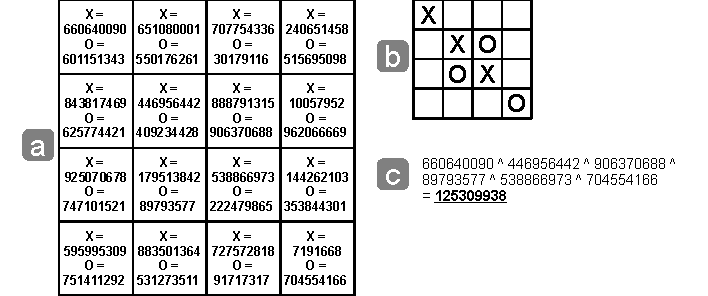
\includegraphics[scale = 1.3]{inhalt/abbildungen/zobrist_hash_tictactoe.pdf}
  \caption{Zobrist Hashing von Spielzuständen.}
  \label{fig:zobrist_hash_tictactoe}
\end{figure} 


In Abbildung \ref{fig:zobrist_hash_tictactoe} wird das Zobrist Hash Verfahren auf einen bestimmten Spielzustand (b) angewendet. Schritt 1: (a) wir weisen jedem Spielfeld zwei zufällige ganzzahlige Werte zu, im Bereich von 0 bis maximal $1 \times 10^{9}$. Einen zufälligen Wert für den Kreuzspielstein an dieser Position und einen für den Kreisspielstein. Das 4x4 Tic Tac Toe Spielbrett sollte insgesamt 32 verschiedene Werte erhalten. Spielsituation (b) soll in einen Zobrist-Hash umgewandelt werden. \\

Der Zobrist-Hash berechnet sich wie folgt (c), ist die aktuelle Position mit einem Kreuzspielstein oder einem Kreisspielstein besetzt, dann wähle den entsprechenden Wert aus der Werttabelle (a). Dies wiederhole für jedes besetzte Spielfeld. Wir verknüpfen die bestimmten Werte, mittels eines exklusiven bzw. bitweisen Oder (XOR). Das Ergebnis ist eine Adresse, die exakt den Spielzustand (b) referenziert. \\


